\section{Requerimientos de un Sistema con Tolerancia a Fallas}

A partir de los distintos casos presentados, en esta sección se busca relevar cuáles son las características comunes en sistemas con tolerancia a fallas. Se analizan las distintas alternativas y luego se mencionan los criterios tenidos en cuenta para el desarrollo de la computadora de vuelo. En este trabajo no se define a priori cuál es la arquitectura del sistema en cuanto al uso de redundancias, por lo que la computadora de vuelo debe tener cierta diversidad en cuanto a sus capacidades.\\

\subsection{Requerimientos Comunes en Sistemas con Redundancias}

Todos los trabajos y ejemplos presentados en la sección anterior comparten la característica de implementar la tolerancia a fallas utilizando varias copias del mismo elemento de hardware. Estas copias trabajan en paralelo y se comparan los resultados obtenidos por cada una de ellas. Las fallas se detectan cuando ocurre una diferencia en los resultados de las copias.\\

{\color{red} EXPLICAR Y JUSTIFICAR EL POR QUÉ DE LAS REDUNDANCIAS POR SOBRE EL USO DE COMPONENTES DE ALTÍSIMA CALIDAD, EN UN PÁRRAFO.}

A continuación, se describen algunas de las características detectadas.

\subsubsection{Sincronismo de los Nodos}

Prácticamente en todos los trabajos presentados se menciona que los nodos reundantes trabajan de manera sincronizada. Esta necesidad surge debido a que las comparaciones se realizan sobre variables que cambian en el tiempo y que tienen validez solamente durante un período de tiempo. Esto es algo característico de sistemas de tiempo real, ya que un dato de un sensor $X(t)$ solamente tendrá validez durante un breve período de tiempo. 
%En las arquitecturas antes presentadas, se menciona que se realiza una comparación de los resultados calculados por cada nodo, para detectar/enmascarar errores. Para que el funcionamiento de esta comparación sea adecuado, los nodos deben estar sincronizados. Esto es un requerimiento para sistemas de tiempo real, como el caso de la computadora de vuelo de un UAV.
En la figura \ref{fig:3_4_1_sincronizacion} se muestra un ejemplo. En el instante $t$, se presenta una nueva medición de un sensor a las tres computadoras de vuelo. Al comienzo de la misión, todas ellas estarán sincronizadas y generarán un resultado del cálculo de la ley de control que corresponde al mismo intervalo de tiempo. Luego, se realiza la votación para elegir el valor correcto. La figura \ref{fig:3_4_1_sincronizacion_2}, muestra lo que sucede al cabo de un período de tiempo. Se presenta una nueva medición de un sensor en el instante $t$. Debido a la desincronización, es posible que las computadoras de vuelo no presenten sus resultados al árbitro a tiempo, por lo que este asumirá que una de las FCCs no presentó ninguna respuesta. Este caso suele estar contemplado dentro de las posibilidades y correpsonde al caso en el que una computadora de vuelo presentó un error y debido a ello no respondió con ningún valor (por ejemplo, se reinició su procesador debido a un \textit{watchdog}). En esos casos el árbitro simplemente asume algún valor por defecto.

\begin{figure}[H]
    \centering
    \begin{subfigure}[b]{0.49\textwidth}
        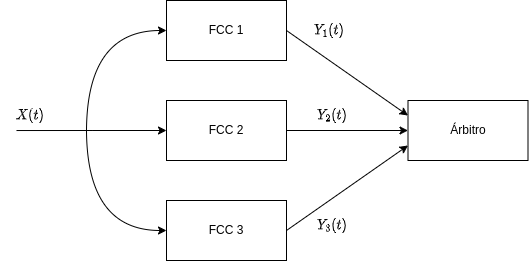
\includegraphics[width=\textwidth]{img/3_4_1_sincronizacion_1.png}
        \caption{Computadoras de vuelo al inicio de la misión.}
        \label{fig:3_4_1_sincronizacion_1}
    \end{subfigure}
    \begin{subfigure}[b]{0.49\textwidth}
        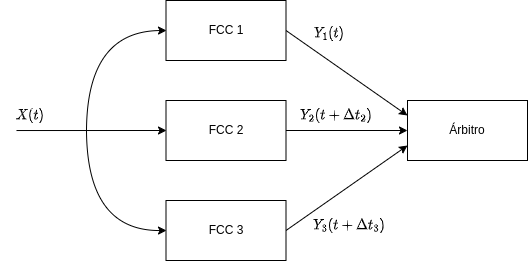
\includegraphics[width=\textwidth]{img/3_4_1_sincronizacion_2.png}
        \caption{Al cabo de un período de tiempo, se desincronizarán.}
        \label{fig:3_4_1_sincronizacion_2}
    \end{subfigure}
    \caption{A medida que transcurra el tiempo, la desincronización entre FCCs impactará en el sistema redundante.}
    \label{fig:3_4_1_sincronizacion}
\end{figure}

Otra situación que puede presentarse, es que los resultados propuestos por las computadoras de vuelo $Y_1$, $Y_2$ e $Y_3$ correspondan a intervalos de tiempo distintos. Este caso es todavía peor que el anterior, ya que no se encuentra contemplado y el árbitro simplemente realizará la votación asumiendo que el dato es válido.

\begin{figure}[H]
    \centering
    \begin{subfigure}[b]{0.49\textwidth}
        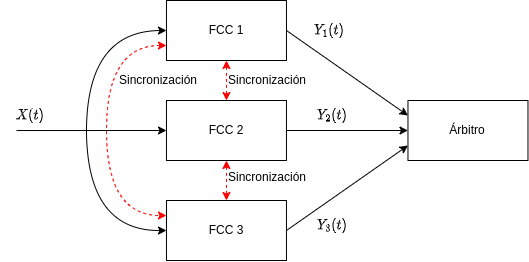
\includegraphics[width=\textwidth]{img/3_4_1_sincronizacion_3.png}
        \caption{Las mismas computadoras de vuelo se encargan de la sincronización.}
        \label{fig:3_4_1_sincronizacion_3}
    \end{subfigure}
    \begin{subfigure}[b]{0.49\textwidth}
        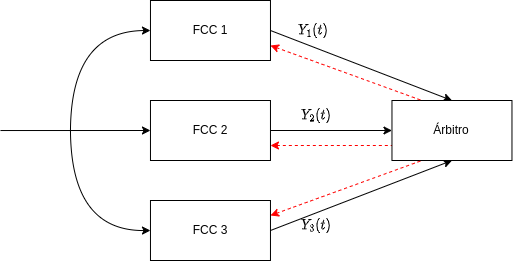
\includegraphics[width=\textwidth]{img/3_4_1_sincronizacion_4.png}
        \caption{En este caso, la sincronización es administrada por el árbitro.}
        \label{fig:3_4_1_sincronizacion_4}
    \end{subfigure}
    \caption{La sincronización entre nodos es necesaria para un correcto funcionamiento de las redundancias.}
\end{figure}

Se concluye que es mandatorio utilizar alguna técnica de sincronización entre los nodos. Como detalle de la figura \ref{fig:3_4_1_sincronizacion_3}, se muestra que la sincronización entre nodos presupone otro canal de comuniación más. Otra forma podría ser relegar la tarea de la sincronización al árbitro, aunque esto nuevamente presenta un punto singular de falla. Como se demostró en esta sección, el sincronismo es un aspecto crítico en el sistema redundante, por lo que se prefiere evitar esto último. Aunque de todas formas quisiera relegarse la sincronización al árbitro, este no solo recibirá mensajes de cada una de las FCCs, sino que además les enviará mensajes. Esto se muestra en la figura \ref{fig:3_4_1_sincronizacion_4}.

\subsubsection{Consenso}\label{sec:consenso}

Como se mostró en la figura \ref{fig:3_4_1_sincronizacion_3}, las computadoras de vuelo pueden comunicarse entre ellas para lograr una sincronización, por ejemplo compartiendo a sus pares un valor asociado a su propio clock interno. Cada FCC propone un valor distinto y estas buscarán ponerse de acuerdo en un valor único. Para que cada una de ellas llegue a la misma conclusión acerca del valor de clock correcto, si todas ellas ejecutan el mismo algoritmo y poseen los mismos valores de entrada, luego llegarán a la misma conclusión. En la figura \ref{fig:3_4_2_consenso_4} se muestra un caso en el que una de las computadoras de vuelo comparte valores de clock distintos a sus pares.

\begin{figure}[H]
    \centering
    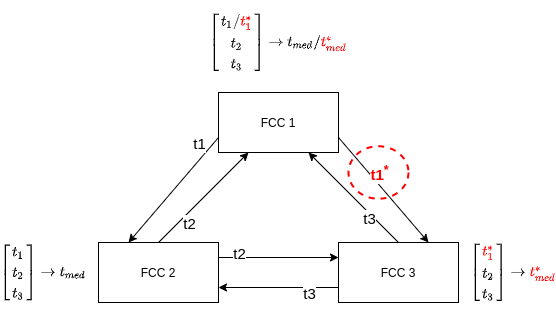
\includegraphics[width=0.6\textwidth]{img/3_4_2_consenso_4.png}
    \caption{La FCC1 entrega un valor distinto de timing a las demás FCCs}.
    \label{fig:3_4_2_consenso_4}
\end{figure}

En este escenario, la FCC1 entrega dos valores distintos de su clock a las demás FCCs. Cada una de ellas luego realiza un promedio para llegar a un único valor. Lo que se observa es que las FCC2 y FCC3 calcularán un valor promedio distinto, es decir, no se sincronizarán.
Una posible solución podría ser que las FCCs hagan un nuevo intercambio, con los valores promedio calculados y realicen una votación interna. Esto se muestra en la figura \ref{fig:3_4_2_consenso_5}.

\begin{figure}[H]
    \centering
    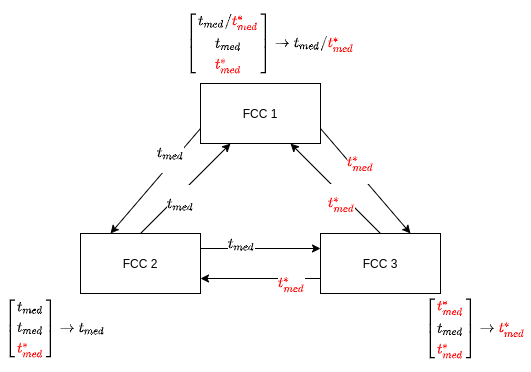
\includegraphics[width=0.6\textwidth]{img/3_4_2_consenso_5.png}
    \caption{Luego de calcular los promedios, las FCCs intercambian sus resultados. Nuevamente, la FCC1 comete una falla en el envío del dato.}
    \label{fig:3_4_2_consenso_5}
\end{figure}

Esta última situación, donde la FCC1 nuevamente comparte dos valores distintos a las demás, puede llevar a que las computadoras de vuelo no se sincronicen, algo que como ya se mencionó, es crítico para la correcta ejecución del algoritmo de tolerancia a fallas.\\

Podría argumentarse que es demasiado pesimista pensar que la FCC1 puede producir la misma falla 2 veces de manera consecutiva, ya que existe una baja probabilidad de que ello suceda. Sin embargo, la situación planteada en esta sección puede tratarse como un tipo de falla típicamente denominada falla bizantina, y que corresponde al caso de fallas de hardware que se manifiestan como comportamientos arbitrarios.\\

Que exista una sincronización entre nodos redundantes implica que estos llegan a un consenso del paso del tiempo y el ritmo al que deben ejecutar sus tareas asignadas. Este consenso resulta crítico para que el sistema pueda detectar fallas correctamente.\\

En cuanto al caso de la figura \ref{fig:3_4_1_sincronizacion_4}, 

\textbf{{\color{red} COMPLETAR}}

\subsection{Uso de Componentes COTS}

\textbf{{\color{red} COMPLETAR}}